\newlecture

\setcounter{section}{3}

%\def\textbookchapter{Chapter 12: Vector Calculus}
\def\coursetopicnumber{IV}
\def\topic{Path-Independent Vector Fields and the Fundamental Theorem of Calculus for Line Integrals} % this is the printed title
\def\shorttopic{Path independence, FTCLI} % short topic
\def\textbookname{Active Calculus} % this is the corresponding textbook
\def\shorttextbookname{AC} % this is the short name for the book
\def\textbooksection{12.4} % corresponding textbook section
\def\textbooksectionurl{https://activecalculus.org/vector/S_Vector_FTCLI.html} % URL for textbook section
\def\handoutday{} % this is the printed date

%%%%%%%%% DOCUMENT CONTENT STARTS BELOW

\thispagestyle{plain}
\topstuff
\section{\topic{} \booklink{}}
\label{sec:ftcli}

\subsection{Line integrals via potential functions}
In Section~\ref{sec:compute-line-integral}, we computed the line integral of $\vec{F}(x,y)=\langle 5-2x,\,\sin(y)\rangle$ along a path $C$ that started at $(0,0)$ and ended at the point $(2,0)$. We broke the path up into two parts, parametrized each part, computed a line integral for each part, added the results, and concluded $\int\limits_C\vec{F}\dotp\dvr = 6$. Revisiting this problem will lead to a nice result.

\begin{ex}\label{ex:sec-12.4-motivating-ex}
    For $\vec{F}(x,y)=\langle 5-2x,\sin(y)\rangle$, suppose $\vec{r}(t)=\langle x(t),\,y(t)\rangle$, for $a\le t\le b$, is a smooth path from $P=(0,0)$ to $Q=(2,0)$. (In particular, $\vec{r}(a)=\langle x(a),y(a)\rangle = \langle 0,0\rangle$ and $\vec{r}(b)=\langle x(b),y(b)\rangle = \langle 2,0\rangle$.) Write out $\int\limits_C\vec{F}\dotp\dvr$ as an integral involving $t$.
\end{ex}

\vfill

\begin{ex}
    Suppose $f$ is a function of $x$ and $y$, and suppose that $x$ and $y$ are each functions of $t$. Thus, $f$ is a function of $t$. What does the chain rule say about $\dfd{f}{t}$?
\end{ex}

\vfill

\begin{ex}
    Let $f(x,y)=5x-x^2-\cos(y)$, $x=x(t)$, and $y=y(t)$. Compute $\dfd{f}{t}$.
\end{ex}

\vfill

\begin{ex}
    Evaluate the integral in Exercise~\ref{ex:sec-12.4-motivating-ex}.
\end{ex}

\vfill

\pagebreak 

\begin{ex}
    On the previous page, we began with the vector field $\vec{F}(x,y)=\langle 5-2x,\,\sin(y)\rangle$. Once we knew about the function $f(x,y)=5x-x^2-\cos(y)$, we could quickly evaluate the line integral. Where did this function come from?
\end{ex}

\vspace{1in}

We first saw the following definition in Section~\ref{sec:vector-fields} when we learned about vector fields.

\begin{defn}[Potential function]
    Given a vector field $\vec{F}(x,y)$ (or $\vec{F}(x,y,z)$), if $f(x,y)$ (or $f(x,y,z)$) is a scalar-valued function such that $\nabla f = \vec{F}$, then $f$ is a \emph{potential function} for $\vec{F}$. When this occurs, we say that $\vec{F}$ is a \emph{gradient vector field}.
\end{defn}

\bigskip 

If $f(x,y)$ is a potential function for $\vec{F}(x,y)$, then $\vec{F}(x,y)=\langle f_x(x,y),\, f_y(x,y)\rangle$. The line integral of $\vec{F}$ over a path $C$ parametrized by $\vec{r}(t)=\langle x(t),\,y(t)\rangle$ for $a\le t\le b$ is
\begin{align*} 
    \int\limits_C\vec{F}\dotp\dvr 
    &=\int\limits_a^b\vec{F}(\vec{r}(t))\dotp\vec{r}\,'(t)\dt\\
    &= \int\limits_a^b \left\langle f_x(x(t),y(t)),\, f_y(x(t),y(t))\right\rangle\dotp\left\langle x'(t),y'(t)\right\rangle\dt \\
    &= \int\limits_a^b \phantom{\left[ f_x(x(t),y(t))x'(t) + f_y(x(t),y(t))y'(t)\right]\dt}
\end{align*}
and 
\[
    \dfd{}{t}\left[f(x(t),y(t))\right]
    = \phantom{f_x(x(t),y(t))x'(t) + f_y(x(t),y(t))y'(t).}
\]
\medskip 

We have an antiderivative for our $\dt$ integral! By the Fundamental Theorem of Calculus from Calculus I/II, we can evaluate the $\dt$ integral by evaluating our antiderivative at the end point minus our antiderivative at the start point:
\[
    \int\limits_C\vec{F}\dotp\dvr 
    = f(x(t),y(t))\Bigg|_{t=a}^{t=b} 
    = \phantom{f(x(b),y(b))-f(x(a),y(a)).}
\]

This is the first fundamental theorem of vector calculus.

\begin{thm}[Fundamental Theorem of Calculus for Line Integrals (FTCLI)]
    For a vector field $\vec{F}$ and a scalar-valued function $f$, if $\vec{F}=\nabla f$ and $C$ is a piecewise-smooth curve from the point $P$ to the point $Q$ parametrized by $\vec{r}(t)$, then
    \[
        \int\limits_C \vec{F} \dotp \dvr = \phantom{f(B)-f(A).}
    \]
\end{thm}

\vspace{1in}

\begin{ex}
    Working with $\vec{F}(x,y)=\langle 5-2x,\,\sin(y)\rangle$ again, let $C$ be the path consisting of line segments from $(1,0)$ to $(4,3)$ to $(-7,1/2)$ to $(0,\pi)$. Evaluate $\int\limits_C\vec{F}\dotp\dvr$.
\end{ex}

\vfill

\subsection{Consequences of FTCLI}
Suppose $C_1$ and $C_2$ are two paths from a point $P$ to a point $Q$. If $\vec{F}$ is a gradient vector field, then the Fundamental Theorem of Calculus for Line Integrals says that, for a potential function $f$ of $\vec{F}$,
\[
    \int\limits_{C_1}\vec{F}\dotp\dvr = \phantom{f(Q)-f(P)}\quad \text{ and } \quad \int\limits_{C_2}\vec{F}\dotp\dvr = \phantom{f(Q)-f(P)}
\]
In other words, the result will be $f(Q)-f(P)$ for any path! To compute the line integral of a gradient vector field over a path, we just need to know the endpoints.
\bigskip 

\begin{defn}[Path-Independent Vector Field]
    Let $\vec{F}$ be a vector field. Suppose that for any points $P$ and $Q$, and any two piecewise-smooth paths $C_1$ and $C_2$ which both start at $P$ and end at $Q$, we always have
    \[
        \int\limits_{C_1}\vec{F}\dotp\dvr 
        = \phantom{\int\limits_{C_2}\vec{F}\dotp\dvr.}
    \]
    When this occurs, we say $\vec{F}$ is \emph{path-independent}.
\end{defn}

\bigskip 

\begin{defn}[Conservative Vector Field]
    Let $\vec{F}$ be a vector field. Suppose that for any piecewise-smooth, closed curve $C$, we always have
    \[
        \int\limits_C\vec{F}\dotp\dvr 
        = 0.
    \]
    When this occurs, we say $\vec{F}$ is \emph{conservative}.
\end{defn}

\bigskip 

\begin{thm}
    For a vector field $\vec{F}$, the following are equivalent statements:
    \begin{itemize}
        \item $\vec{F}$ is a gradient vector field;
        \item $\vec{F}$ is a path-independent vector field;
        \item $\vec{F}$ is a conservative vector field.
    \end{itemize}
\end{thm}


\pagebreak 

\subsection{Some notation}
Our definitions motivate some handy notation for line integrals.

First, if $\vec{F}$ is a path-independent vector field, then we can write 
\[
    \int\limits_P^Q\vec{F}\dotp\dvr
\]
to mean the line integral of $\vec{F}$ over a path $C$ that goes from $P$ to $Q$. (Note that this only makes sense if $\vec{F}$ is path-independent!)
\medskip 

Second, if $C$ is a closed curve (same start and end point), we can write the line integral of $\vec{F}$ over $C$ as
\[
    \oint\limits_C\vec{F}\dotp\dvr.
\]
A line integral over a closed curve is often referred to as \emph{circulation}.

\bigskip 

\begin{thm}[Circulation of a gradient vector field]
    Suppose $\vec{F}$ is a gradient vector field and $C$ a closed curve. Then the circulation of $\vec{F}$ over $C$ is 
    \[
        \oint\limits_C\vec{F}\dotp\dvr = \phantom{0.}
    \]
\end{thm}

\begin{ex}
    Here are the two vector fields $\vec{F}(x,y)=\left\langle -y/4,\, x/4\right\rangle$ and $\vec{G}(x,y)=\langle x/3,0\rangle$ from the start of Section~\ref{sec:vector-fields}. Is $\vec{F}$ a gradient vector field? If $\vec{G}$ a gradient vector field?
    
    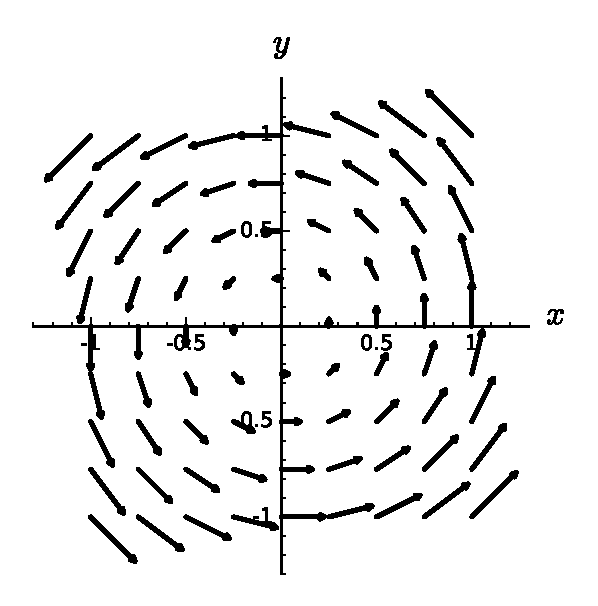
\includegraphics[width=.35\textwidth]{images/vf1.eps} \hfill 
    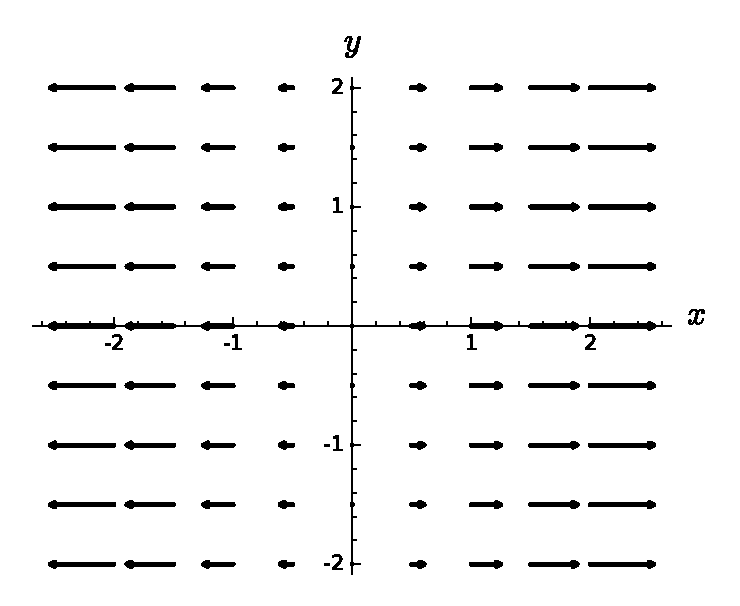
\includegraphics[width=.4\textwidth]{images/vf2.eps}\label{img:sage-vector-field-5}
\end{ex}

\vfill 

\begin{ex}
    Does the vector field $\vec{F}(x,y)=\langle -y/4,\, x/4\rangle$ have a potential function?
\end{ex}

\vspace{.5in}

\pagebreak 

\subsection{How to tell if a potential function exists}
\begin{ex} 
    At the end of Section~\ref{sec:vector-fields}, we asked whether the vector field $\vec{F}(x,y)=\langle y,\, 3\rangle$ has a potential function. We were unable to find one. Use Clairaut's Theorem to explain why this vector field doesn't have a potential function.
\end{ex}

\vspace{3in}

\noindent This leads to the ``curl test.'' (The \emph{curl} of a vector field, which we won't see in this course, essentially measures how an object in a 3D vector field will rotate as it moves.)

\begin{thm}[The ``curl test,'' 2D version]
    For a vector field $\vec{F}(x,y)=\left\langle F_1(x,y), F_2(x,y)\right\rangle$,
    $\vec{F}$ is a gradient vector field if and only if 
    \[
        \phantom{\pd{F_2}{x}=\pd{F_1}{y}.}
    \]
\end{thm}

\vspace{.5in}

For a function of three variables, we have more mixed partials to think about! Clairaut's Theorem says $f_{xy}=f_{yx}$, $f_{xz}=f_{zx}$, and $f_{yz}=f_{zy}$. This leads to a ``curl test'' for a 3D vector field.

\begin{thm}[The ``curl test,'' 3D version]
    For a vector field 
    \[
        \vec{F}(x,y,z)
        =\left\langle F_1(x,y,z),\, F_2(x,y,z),\, F_3(x,y,z)\right\rangle,
    \]
    $\vec{F}$ is a gradient vector field if and only if all three of the following hold:
    \[
        \phantom{\pd{F_2}{x} = \pd{F_1}{y}, \quad \pd{F_3}{x} = \pd{F_1}{z}, \quad  \pd{F_2}{z} = \pd{F_3}{y}.}
    \]
\end{thm}

\pagebreak 

\begin{ex}
    Let $\vec{F}=\left\langle xyz,\,x^2e^z,\,x^2yz^2\right\rangle$, and let $\vec{G}=\left\langle ye^x+2xz,\,e^x,\,\cos{z}+x^2\right\rangle$.
    \begin{enumerate}
        \item Use the curl test to determine whether $\vec{F}$ and/or $\vec{G}$ is a gradient vector field.
        \item Let $C$ be parametrized by 
        $\vec{r}(t) = \left\langle \sin^3(t),\, \frac{2t}{\pi}\cos^4(t),\, t\right\rangle$
        for $0\le t\le \pi$. Evaluate one of the following (your choice): $\displaystyle\int\limits_C\vec{F}\dotp\dvr$ or $\displaystyle\int\limits_C\vec{G}\dotp\dvr$.
    \end{enumerate}
\end{ex}

\vfill 

If we know that a vector field has a potential function, we will typically be able to think about integrating each component of the vector field in the relevant variable and piece the results together to get a potential function. (And, of course, we can always check to see if we're right!) For a more concrete method to follow, see Example 2 in \href{https://tutorial.math.lamar.edu/Classes/CalcIII/ConservativeVectorField.aspx}{Paul's Notes, Section 5-6: Conservative Vector Fields}.
%\vspace{.2in}

